% =====================================================================
%  Draft 4 (his vocabulary), 21 Oct 2026: same content as Draft 3, word choice
%  and argument shape moved to his own corpus (see VOCAB_MAP.md, NOTES.md).
%  Draft 3 (his voice), 21 Oct 2026: same content as Draft 2, prose reworded
%  in Mohammed Shehzaad Khan's own voice (see STYLE_PROFILE.md, NOTES.md).
%  Every fact, number, citation, label, TBD and comment below is unchanged.
%  Draft 2 Research Paper of This Project (21 Oct 2026)
%  E.C.H.O  (Efficient Contextualized History Orchestrator)
%
%  Built on the official IEEE Conference Template (IEEEtran, conference
%  mode, two columns). Upload this file as main.tex to Overleaf and it
%  compiles with pdfLaTeX without any other files (both figures are TikZ).
%
%  Draft 2 notes for the team:
%   * The paper describes the FINAL system as designed and decided on
%     2026-10-21 (decision ids A1..A43 in docs/review/ste_open_items.md),
%     not only the current build. Build runs Thu 22 to Sun 25 Oct 2026.
%     Claims beyond the current build (must be finished before submission):
%       - agentic retrieval loop: search_memories tool, up to 5 rounds,
%         usually 2 / max 6 LLM calls (A26); chat answers with memory pills
%         and a moment strip (A27); streamed progress over SSE (A28)
%       - local PostgreSQL + local Redis, schema opened (A31); visit table
%         for Chrome/YouTube with dwell per visit (A1.1, A1.1b); stored
%         tsvector + GIN index over the full text (A24.3)
%       - attachment text extracted at ingestion, incl. XLSX, PPTX, EML and
%         Tesseract OCR (A4, A22); query matched passages only (A23, A24.2)
%       - Gmail incremental polling with history.list, Spam/Trash skipped
%         (A5, A38); hidden preview text dropped, body parts joined (A6);
%         signature removal deleted (A12); inline replies kept (A14.2)
%       - Chrome: headings from the extension (A13), 38 word sensitive list
%         with whole token matching, secret query keys stripped, stricter
%         form check (A7), 7 app domains + public sections, rules served by
%         GET /chrome/rules (A9), Gmail web skipped (A9.1), app page minimum
%         on the server (A8.2), link clicks no longer count (A39 part 2)
%       - A39 timings (scroll 15 %, Shorts 10 s, completion 10 % with 5 s
%         floor, KNN from 5 items); YouTube 5 s revisit check (A34)
%       - Stage 3 richer seeds + seed threshold (A18), balanced recompute
%         (A20), recompute at worker start (A36), Stage 4 via Decisions API
%         on OpenAI (A21), curated domain map growth (A17)
%       - effort score: median for unread mail (A29); KNN only suggestion
%         threshold (A32); retention setting (A37); popup pause toggle (A33)
%       - automatic retry of failed enrichment items (carried over from
%         Draft 1; NOT scheduled by any decision, today manual via
%         ENP_RETRY_FAILED)
%   * Still open on 2026-10-21: A16 (embedding token budget), A40
%     (embedding model, \embmodel below), A42 (auto accept), A43 (user
%     groups under system groups), A11 outcome (transcripts, decided Thu).
%   * No measured results. Every number still to be measured is a visible
%     \tbd{...} placeholder. Search the PDF for "TBD".
%   * Style: plain wording, no hyphens or dashes in prose, US spelling.
% =====================================================================
\documentclass[conference]{IEEEtran}
\IEEEoverridecommandlockouts
% The preceding line is only needed to identify funding in the first footnote. If that is unneeded, please comment it out.
\usepackage{cite}
\usepackage{amsmath,amssymb,amsfonts}
\usepackage{algorithmic}
\usepackage{graphicx}
\usepackage{textcomp}
\usepackage{xcolor}
\usepackage{url}
\usepackage{array}
\usepackage{tikz}
\usetikzlibrary{arrows.meta,positioning,fit,calc}
% No automatic hyphens at line ends (style rule for this paper)
\hyphenpenalty=10000
\exhyphenpenalty=10000
\emergencystretch=1.5em
% Author layout: two authors per row, first author flush with the left margin.
\makeatletter
\newcommand{\authorflushleft}{\end{@IEEEauthorhalign}\hskip 0pt plus -1fill\begin{@IEEEauthorhalign}}
\newcommand{\linebreakand}{\end{@IEEEauthorhalign}\par\noindent\mbox{}\begin{@IEEEauthorhalign}}
\makeatother
\def\BibTeX{{\rm B\kern-.05em{\sc i\kern-.025em b}\kern-.08em
    T\kern-.1667em\lower.7ex\hbox{E}\kern-.125emX}}

% ---------------------------------------------------------------------
% One line swaps. Change a model name HERE only.
% TODO A40: embedding model not decided yet. Leading candidate below
% (384 dimensions, 8192 token window). Today's code still runs
% all-MiniLM-L6-v2 (enp/embedding_generator.py:56), also 384 dimensions.
\newcommand{\embmodel}{\texttt{granite\allowbreak-embedding\allowbreak-small\allowbreak-english\allowbreak-r2}}
\newcommand{\embdim}{384}
% Cross encoder (rse/config.py CROSS_ENCODER_MODEL). A40 may change it too.
\newcommand{\rerankmodel}{\texttt{ms\allowbreak-marco\allowbreak-MiniLM\allowbreak-L\allowbreak-6\allowbreak-v2}}
% Hosted LLM (decision A25, rse/config.py LLM_CONFIG).
\newcommand{\llmname}{GPT\nobreakdash-5.6 Luna}
% Visible placeholder for anything not yet measured or decided.
\newcommand{\tbd}[1]{\textbf{[TBD: #1]}}
% ---------------------------------------------------------------------

% Shared style for the diagrams
\tikzset{
  box/.style={draw, rounded corners=2pt, align=center, font=\footnotesize,
              minimum height=6mm, inner sep=3pt, fill=white},
  store/.style={box, fill=gray!12},
  llm/.style={box, fill=gray!28, font=\footnotesize\bfseries},
  arr/.style={-{Stealth[length=2mm]}, semithick},
  grp/.style={draw, dashed, rounded corners=3pt, inner sep=4pt}
}

\begin{document}

\title{E.C.H.O: An Intent Aware Personal Memory System for Unified Search Across Email, Web, and Video History}

\author{\authorflushleft\IEEEauthorblockN{1\textsuperscript{st} Arjun Sai N}
\IEEEauthorblockA{\textit{Dept. of Computer Science and Engineering} \\
\textit{PES University}\\
Bengaluru, India}
\and
\IEEEauthorblockN{2\textsuperscript{nd} Mohammed Mir Fazlai Ali}
\IEEEauthorblockA{\textit{Dept. of Computer Science and Engineering} \\
\textit{PES University}\\
Bengaluru, India}
\linebreakand
\IEEEauthorblockN{3\textsuperscript{rd} Mohammed Shehzaad Khan}
\IEEEauthorblockA{\textit{Dept. of Computer Science and Engineering} \\
\textit{PES University}\\
Bengaluru, India}
\and
\IEEEauthorblockN{4\textsuperscript{th} Mrigank Jain}
\IEEEauthorblockA{\textit{Dept. of Computer Science and Engineering} \\
\textit{PES University}\\
Bengaluru, India}
\linebreakand
\IEEEauthorblockN{5\textsuperscript{th} Mannuru Shalima Sulthana}
\IEEEauthorblockA{\textit{Dept. of Computer Science and Engineering} \\
\textit{PES University}\\
Bengaluru, India}
}

\maketitle

\begin{abstract}
In a single day, a person meets information in many places: the inbox, the browser, and video sites. Each place keeps its own history behind its own search box, so finding something again starts with guessing where it was seen. We present E.C.H.O (Efficient Contextualized History Orchestrator), a personal memory for a single user. It collects Gmail, Chrome, and YouTube activity into one store on the user's own laptop and answers questions about it in plain language. All mail is kept, except what Gmail itself files as spam or trash. A web page or a video, though, is kept only when signals such as foreground time, scrolling, watch time, or a return visit show that the person actually attended to it. In the background, a worker then cleans each item and pulls text out of its attachments. It also assigns one of five broad categories and embeds the item for search by meaning. A question goes to a language model that may call a single search tool, which is plain code. This tool runs keyword and vector search together and fuses the two ranked lists by reciprocal rank fusion. It widens the search when the results look weak, and it reorders the survivors with a local cross encoder. A typical question costs two model calls, and the code allows at most six. Storage, indexing, and search all run locally. The model receives the question and short excerpts, but not whole emails, pages, or transcripts. Also, a wellbeing module describes how time is spent without judging it, and it sorts items into personal goals only with the user's approval. This paper explains the design and the evaluation protocol, and the measured results will follow.
\end{abstract}

\begin{IEEEkeywords}
personal information management, retrieval augmented generation, hybrid search, reciprocal rank fusion, tool calling agents, intent aware capture, local first software, digital wellbeing
\end{IEEEkeywords}

% ---------------------------------------------------------------------
\section{Introduction}
% ---------------------------------------------------------------------
Suppose a student is preparing for a job interview. The company sends an email, and over the following days the student reads articles about operating systems in Chrome and watches a few tutorials on YouTube. A week later, the student wants that material back. Now the email sits in Gmail and the videos sit in the YouTube watch list, while the articles are buried in the browser history. Each of these apps has its own search box, and none of them knows about the other two. So the student either searches all three, one at a time, or starts again from scratch.

The idea of a machine that remembers what its owner has seen is not new. Bush called it the memex in 1945 \cite{b1}, and later systems such as Stuff I've Seen \cite{b2} and MyLifeBits \cite{b3} built personal stores of mail, pages, and documents. But two problems still stand in the way of daily use. The first problem is noise. A browser logs every page that opens, including stray clicks and tabs closed after two seconds. So a memory built directly on that log fills up with things nobody read. The second problem is recall by exact words. A search box needs the right keyword, while people remember loosely, as in ``the OS material I read after the interview email.''

E.C.H.O tackles both problems. It watches Gmail, Chrome, and YouTube, but it keeps a page or a video only when engagement shows real attention. All items share one data model on the user's laptop, where they are enriched in the background and can be queried in natural language. Every answer is grounded in the stored items, following retrieval augmented generation \cite{b4}.

The main contributions are:
\begin{itemize}
\item An intent aware capture layer with a separate rule set for each source, along with privacy filters that act before anything is stored. Here, sensitive pages lose their text and secret parameters are cut from addresses, and private work apps contribute only a page title.
\item A local storage model in which emails, pages, and videos share one central table. PostgreSQL is the permanent record, Redis holds short lived state, and the FAISS index can be rebuilt from PostgreSQL. Attachment text is already extracted when the mail arrives, so it is searchable as well.
\item A bounded agentic retrieval loop. The language model plans and phrases the searches, while a deterministic tool does the actual searching. This tool runs hybrid keyword and vector search, rank fusion, a rule based quality check with widening, and cross encoder reranking. A typical question needs two model calls, and the code sets a hard limit of six.
\item A wellbeing module that reports time, sessions, and self declared regret only in descriptive terms. Along with it comes a grouping engine that files an item under a personal goal only with the user's explicit approval.
\end{itemize}

Section~\ref{sec:related} reviews related work, and Section~\ref{sec:overview} gives an overview of the system. Next, Section~\ref{sec:method} covers capture, storage, enrichment, and retrieval, and Section~\ref{sec:wba} describes the wellbeing module and user groups. Section~\ref{sec:privacy} then covers privacy, and Section~\ref{sec:impl} covers the implementation. The evaluation protocol is in Section~\ref{sec:eval}. Finally, Section~\ref{sec:limits} lists the limitations and Section~\ref{sec:conc} concludes.

% ---------------------------------------------------------------------
\section{Related Work}\label{sec:related}
% ---------------------------------------------------------------------
\subsection{Personal Information Management}
Bush imagined the memex as a desk that holds a person's books, records, and letters and brings any of them back quickly \cite{b1}. Stuff I've Seen built one index over everything a person had already seen, whether an email, a web page, or a document, and used that prior exposure as a cue for search \cite{b2}. MyLifeBits kept personal data in a SQL database, with the aim of storing everything that could be captured \cite{b3}. E.C.H.O shares the same goal of refinding, but it differs in two ways. First, it filters at capture time and does not store everything. Second, it goes a step beyond a query box and answers questions in natural language.

\subsection{Retrieval Augmented Generation and Tool Use}
Retrieval augmented generation couples a retriever with a text generator so that the generated answer draws on the retrieved documents \cite{b4}. E.C.H.O applies this idea to a personal collection and arranges the steps as a graph built with LangGraph \cite{b5}. ReAct showed that a language model can interleave reasoning with actions such as search calls, and that grounding each step in tool output reduces invented facts \cite{b13}. We borrow this pattern, but in a deliberately narrow form. The model has exactly one read only tool, and apart from two small local encoders, that tool contains no model of its own. Also, the number of rounds is capped in the code.

\subsection{Hybrid Search and Reranking}
Sentence embeddings such as Sentence BERT make it possible to compare texts by meaning, using cosine similarity \cite{b6}. E.C.H.O embeds every item with a small local sentence model and searches the vectors with FAISS \cite{b8}. For keyword search, it uses the full text search built into PostgreSQL. The problem is that the two methods score on unrelated scales, so directly adding their scores is not meaningful. Reciprocal rank fusion solves this, as it uses only the position of each item in each list \cite{b9}. After fusion, a cross encoder reads the question and a candidate together and scores how well they match. Nogueira and Cho showed that this works well for passage reranking \cite{b10}. Our cross encoder is a compact MiniLM \cite{b7} model trained on the MS MARCO passage ranking data \cite{b11}.

\subsection{Local First Software}
Kleppmann et al.\ describe local first software, in which users keep ownership of their data and the application works from a copy on their own device \cite{b12}. E.C.H.O follows the same idea, as the database, the vector index, the cache, and both encoders run on the user's laptop. The hosted language model receives only small, chosen pieces of text.

\subsection{Digital Wellbeing Tools}
Lyngs et al.\ reviewed hundreds of digital self control apps and browser extensions and found that most of them block, limit, or track usage against a goal \cite{b14}. E.C.H.O is different from these tools. It shows where the time went and lets the user mark the items they regret, but it does not score the user or block any content. It also does not label time as wasted.

% ---------------------------------------------------------------------
\section{System Overview}\label{sec:overview}
% ---------------------------------------------------------------------
Fig.~\ref{fig:arch} shows the main parts of the system. First, data comes in through three connectors. The Gmail connector reads mail through the Gmail API with OAuth and asks only for the changes since its last check. A Chrome extension observes desktop browsing and YouTube playback, and the YouTube connector then fills in the video details from the YouTube Data API. Every connector hands its items to one FastAPI gateway, where the storage engine writes each item in a single transaction and skips duplicates.

Next, there are three stores, and each has a separate job. PostgreSQL is the permanent record of every item. FAISS holds the embedding vectors, and it can be rebuilt from PostgreSQL. Redis keeps the short lived state, meaning revisit flags, cached text, rate limits, and the user's capture settings. This entire storage layer runs on the user's laptop.

Three modules then work on the stored data. The enrichment worker prepares new items for search in the background, and the retrieval engine answers questions. The wellbeing module turns the stored activity into time summaries, sessions, regret patterns, and group suggestions. The main interface is a React dashboard, along with a small extension popup that lets the user pause capture.

\begin{figure}[t]
\centering
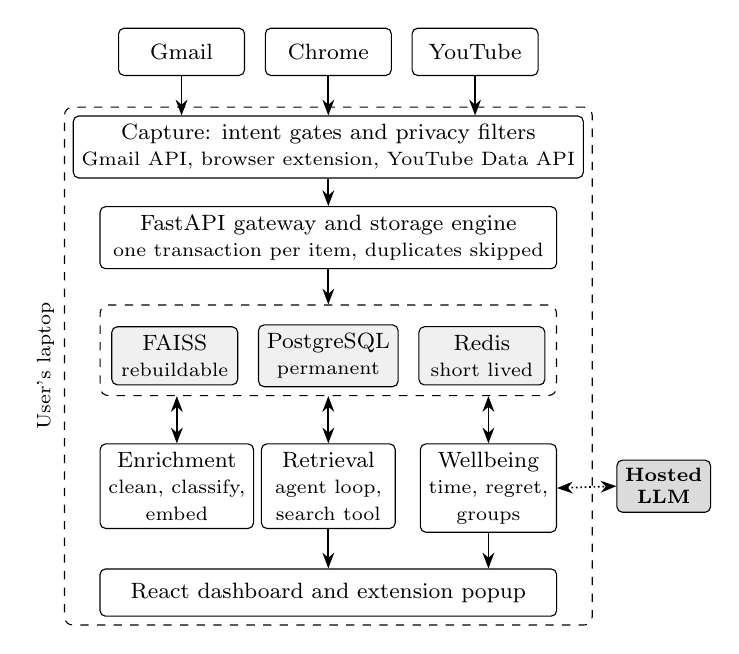
\begin{tikzpicture}[node distance=3.5mm and 2.5mm]
  \node[box, minimum width=16mm] (gm) {Gmail};
  \node[box, minimum width=16mm, right=of gm] (ch) {Chrome};
  \node[box, minimum width=16mm, right=of ch] (yt) {YouTube};
  \node[box, minimum width=58mm, below=5mm of ch] (cap)
      {Capture: intent gates and privacy filters\\ \scriptsize Gmail API, browser extension, YouTube Data API};
  \node[box, minimum width=58mm, below=of cap] (gw)
      {FastAPI gateway and storage engine\\ \scriptsize one transaction per item, duplicates skipped};
  \node[store, minimum width=16mm, below=7mm of gw] (pg) {PostgreSQL\\ \scriptsize permanent};
  \node[store, minimum width=16mm, left=of pg] (fa) {FAISS\\ \scriptsize rebuildable};
  \node[store, minimum width=16mm, right=of pg] (rd) {Redis\\ \scriptsize short lived};
  \node[grp, fit=(fa)(pg)(rd), inner ysep=5pt, yshift=2pt] (st) {};
  \node[box, minimum width=17mm, below=6mm of st.south west, anchor=north west] (enp)
      {Enrichment\\ \scriptsize clean, classify,\\ \scriptsize embed};
  \node[box, minimum width=17mm, below=6mm of st.south, anchor=north] (rse)
      {Retrieval\\ \scriptsize agent loop,\\ \scriptsize search tool};
  \node[box, minimum width=17mm, below=6mm of st.south east, anchor=north east] (wba)
      {Wellbeing\\ \scriptsize time, regret,\\ \scriptsize groups};
  \node[box, minimum width=58mm, below=5mm of rse] (ui) {React dashboard and extension popup};
  \node[grp, fit=(cap)(gw)(st)(enp)(wba)(ui), inner sep=3pt] (lap) {};
  \node[font=\scriptsize, rotate=90, anchor=south] at (lap.west) {User's laptop};
  \node[llm, minimum width=11mm, right=3mm of lap.east |- rse.east, anchor=west, font=\scriptsize\bfseries] (lm) {Hosted\\LLM};
  \draw[arr] (gm) -- (gm |- cap.north);
  \draw[arr] (ch) -- (cap);
  \draw[arr] (yt) -- (yt |- cap.north);
  \draw[arr] (cap) -- (gw);
  \draw[arr] (gw) -- (st.north);
  \draw[arr, {Stealth[length=2mm]}-{Stealth[length=2mm]}] (enp.north) -- (enp.north |- st.south);
  \draw[arr, {Stealth[length=2mm]}-{Stealth[length=2mm]}] (rse.north) -- (rse.north |- st.south);
  \draw[arr, {Stealth[length=2mm]}-{Stealth[length=2mm]}] (wba.north) -- (wba.north |- st.south);
  \draw[arr] (rse) -- (ui);
  \draw[arr] (wba.south) -- (wba.south |- ui.north);
  \draw[arr, densely dotted, {Stealth[length=2mm]}-{Stealth[length=2mm]}] (wba.east) -- (lm.west);
\end{tikzpicture}
\caption{Main parts of E.C.H.O. Everything inside the dashed frame runs on the user's laptop. The dotted arrow is the only path to the hosted language model; it carries short text from three callers (classification, retrieval, weekly reflection), described in Section~\ref{sec:privacy}.}
\label{fig:arch}
\end{figure}

% ---------------------------------------------------------------------
\section{Methodology}\label{sec:method}
% ---------------------------------------------------------------------
\subsection{Intent Aware Capture}
What should E.C.H.O keep? Each source has its own answer, which is summarized in Table~\ref{tab:gates}. These values are the ones chosen for the final system. The browser and the server hold matching copies of them, so that the server does not silently refuse a page that the extension sends.

Gmail is treated differently from the other two sources. Mail arrives on its own and is not chosen by the user. Also, the daily volume is small, and even an unread message may matter later. So every message is stored when it arrives. The connector polls every 30 seconds, but each poll asks Gmail only for the changes since a saved history position. It does not list the entire mailbox each time. If that position has expired, the connector lists the mailbox once, and the uniqueness rule on stored items absorbs the overlap. Mail that Gmail has already filed as spam or trash is not read at all, so Gmail's own spam filter also acts as the spam filter of E.C.H.O. When the user opens a message in Gmail on the web, the extension reports the message id and the seconds spent reading, and nothing else.

A Chrome page passes a two phase gate. In phase one, the page must stay in the foreground for at least five seconds. A page that fails this phase is dropped, and only a page that passes it is remembered for revisit detection. In phase two, at least one sign of attention must appear. This sign can be enough foreground time, enough scrolling, a real interaction, or a visit to the same page within the last 24 hours. Selecting text or clicking inside the page counts as an interaction, but clicking a link does not. This is because a click that leaves the page shows a choice to go elsewhere, and not interest in the page itself. Time is counted only while the tab is active, the window has focus, and the user has not been idle for 30 seconds. Along with the text of the main content, the extension also sends the top level headings of the page. These headings later help the page to be found by its topic.

A YouTube video is kept when the user watches it long enough or watches a large enough share of it. A pause, a seek, a change of speed, or a return to the same video within a day also keeps it. The completion rule requires at least five seconds of real watching, such that swiping past a short clip does not count as watching ten percent of it. Once a video has been watched for five seconds, the extension records the visit, so that a second short visit can pass through the revisit rule. Shorts are recognized from the page address itself, and they have a lower time bar.

\begin{table}[t]
\caption{Capture Rules for Each Source}
\label{tab:gates}
\centering
\renewcommand{\arraystretch}{1.15}
\begin{tabular}{|>{\raggedright\arraybackslash}p{1.35cm}|>{\raggedright\arraybackslash}p{6.2cm}|}
\hline
\textbf{Source} & \textbf{An item is kept when} \\
\hline
Gmail & Always, at arrival, except mail in Spam or Trash. Polled every 30~s for changes only. Reading time is added when a message is opened (opens under 3~s are ignored). \\
\hline
Chrome & Phase 1: at least 5~s in the foreground. Phase 2: any one of at least 10~s in the foreground, at least 15\% scroll depth, one interaction other than a link click, or a revisit within 24~hours. Work app pages: at least 5~s or one interaction, title only. \\
\hline
YouTube & Any one of at least 20~s of foreground playback (10~s for Shorts), at least 10\% of the video watched with at least 5~s of watching, a pause, seek, or speed change by the user, or a revisit within 24~hours. \\
\hline
\end{tabular}
\end{table}

\subsection{Storage Model}
Each email, page, and video becomes one row in a central table of memory items. Fields that belong to a particular source go into a matching table for Gmail, Chrome, or YouTube, and attachments get a table of their own. As engagement counters such as reading time, watch time, and revisits change often, they are kept separately. Also, Chrome and YouTube write one row for every admitted visit, with the time of the visit and the seconds spent. This way, a page read on two different days is counted on both days. The complete schema has 17 tables.
% 17 = the 16 tables in scripts/setup_db.py + the visit table (A1.1).
% Other decided schema changes: gmail_attachments.extracted_text (A4),
% stored tsvector + GIN index (A24.3), classification_confidence dropped
% (A21). A43 (still open) may add user_groups.system_group_id.

A uniqueness rule on the pair of source type and source id stops the same item from being stored twice, for example after a connector restarts. Every item always carries one of the five system groups, and misc is the fallback. Items are first written in a raw state and flagged as unprocessed. This keeps the capture path short and safe against crashes. Later, if a revisited page comes back with different text, it is flagged again so that its vector is rebuilt. Timestamps are stored in UTC and shown to the user in local time.

A user can delete a single item, which hides it from every query. Apart from this, a retention setting lets the user keep items forever, for one year, or for six months. As recalling old things is the whole point of the system, keeping items forever is the default. If the user picks a shorter window, a job at backend startup permanently removes the older items from PostgreSQL, the FAISS index, and Redis together.

\subsection{Background Enrichment}
A background worker picks up the unprocessed items every few seconds. As it runs outside the capture path, a slow enrichment step cannot slow down capture. Each item then goes through four steps.

\textit{Cleaning.} For email, HTML is converted to text with the line breaks kept, and scripts, styles, tracking pixels, and hidden preview text are removed. When the sending app has split a body around an inline image, the parts are joined back together. Quoted earlier messages are removed, but the lines the sender typed between quoted lines are kept. This is because an inline reply is often the most important part of the message. A heuristic remover that we tested cut real body text in six of eight sample messages, while a leftover signature only adds a little noise. So signatures are deliberately left in place, as a little noise is better than lost body text. For a reply, keywords from earlier messages in the same thread are added, so that a terse ``Re:'' can still be found by its topic. For web pages, the extension has already picked the main content and the headings, and the worker separates the headings from the body. A video's text is made of its title, channel, category, tags, description, and transcript. The server fetches the transcript with a transcript library, trying English captions first and automatic captions second. A video without captions is embedded without one.
% TODO A11: transcript source decided Thu 22 Oct (youtube-transcript-api,
% else no transcripts). If it fails, change the sentence above to
% "title, channel, category, tags, and description".

\textit{Attachments.} The same worker extracts attachment text when the mail is processed. It supports PDF, DOCX, XLSX, PPTX, HTML, forwarded messages, and plain text formats such as TXT, CSV, Markdown, JSON, and calendar files. Images and scanned PDFs are read with Tesseract OCR \cite{b15}, while inline images such as signature logos, and very small images, are skipped. The extracted text is stored next to the attachment record and not inside the email body. The beginning of each attachment joins the embedded text of the email, while the entire text joins the keyword index. So content deep inside a file can still be found by keyword.

\textit{Embedding.} The cleaned text is turned into a \embdim{} dimension vector with the \embmodel{} sentence model \tbd{confirm final model, decision A40}. The text is assembled such that the short hints come first. They are the subject, keywords, and sender for mail, the domain and headings for pages, and the channel and category for videos. Long text such as a body or a description comes last. So if the text has to be trimmed to the input window of the model, only the end of the long part is removed \tbd{token budget, decision A16}. The vector is then added to the FAISS index without a rebuild.

\textit{Classification.} Every item receives one of five broad groups, which are work, study, entertainment, personal, and misc. The group is chosen by a four stage cascade. Stage one reads structural signals from the source, such as Gmail category labels, academic mail domains, or the YouTube video category. Next, stage two looks up the web domain in a curated table. Then stage three compares the vector of the item with a center point for each group and accepts only a clear winner. Each center starts as the mean of several example sentences written for its group. While a center is still a seed, it uses a lower acceptance bar \tbd{seed threshold, measured on labeled rows}. Once a group has at least ten confirmed items, its center is recomputed from real items. Each source is weighted equally here, so that a center learns a topic and not the look of one particular source. A recomputed center accepts an item only if the cosine similarity is at least 0.55 and leads the second best group by at least 0.08. The recomputation runs when the worker starts, if the stored centers are missing or older than 30 days. Finally, stage four asks the language model, one item at a time, using only the title and about 300 characters of text. With an OpenAI model, the call is a typed choice among the five group names. With other providers, the reply must be exactly one group name, and any other reply becomes misc. If the typed call raises an error, that item takes the single word path instead, so classification does not stop. No confidence value is stored.

\textit{State tracking.} Each item ends as either processed or failed. Failed items are kept separately and retried automatically, so a failure is not counted as done, and it is not lost either.
% Beyond build (carried over from Draft 1): today retry is manual via the
% ENP_RETRY_FAILED setting; no decision schedules automatic retry yet.

\subsection{Retrieval Loop}
How is a question answered? It passes through the loop in Fig.~\ref{fig:graph}. The language model, \llmname{}, receives the conversation so far, today's date, the question, and one tool called \texttt{search\_memories}. This tool takes a query, and optionally a list of sources, a time phrase, and a sender or domain. The model decides how to phrase the search, and it may issue several searches in parallel in one round, for instance one per source. After reading the results, it either answers directly or searches again. A usual question needs one call that searches and one call that answers. The code allows at most five search rounds. After the fifth round, the next call is made without the tool, such that the model has to answer. So a question costs between two and six model calls, and this bound is enforced by the program, not by the prompt.

\begin{figure}[t]
\centering
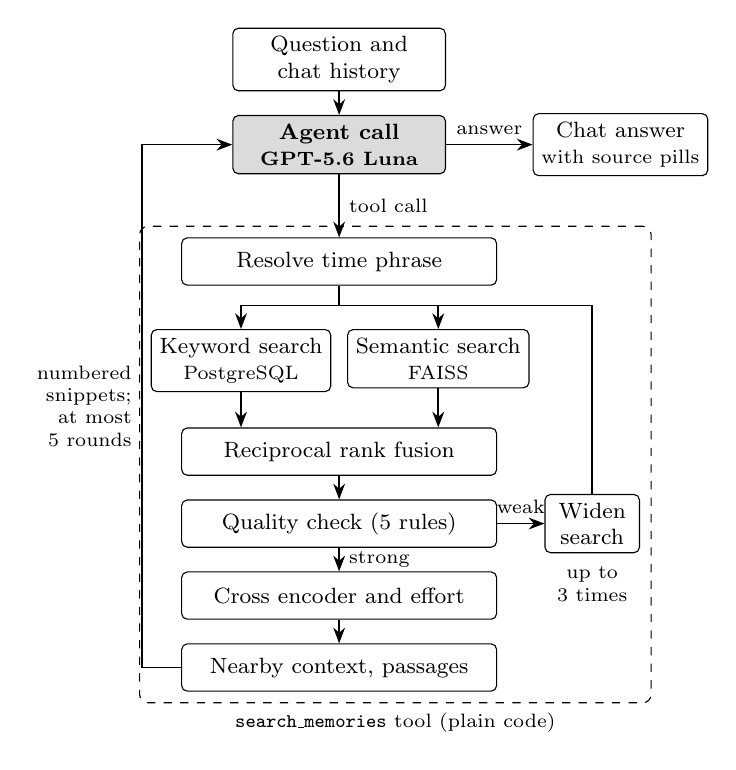
\begin{tikzpicture}[node distance=3mm and 3mm]
  \node[box, minimum width=27mm] (q) {Question and\\ chat history};
  \node[llm, minimum width=27mm, below=of q] (ag) {Agent call\\ \scriptsize\llmname};
  \node[box, minimum width=22mm, right=11mm of ag] (an) {Chat answer\\ \scriptsize with source pills};
  \node[box, minimum width=40mm, below=8mm of ag] (ta) {Resolve time phrase};
  \coordinate (bus) at ($(ta.south)+(0,-2.5mm)$);
  \node[box, minimum width=19mm, anchor=north east] (kw) at ($(bus)+(-1mm,-3mm)$) {Keyword search\\ \scriptsize PostgreSQL};
  \node[box, minimum width=19mm, anchor=north west] (se) at ($(bus)+(1mm,-3mm)$) {Semantic search\\ \scriptsize FAISS};
  \node[box, minimum width=40mm, anchor=north] (rrf) at ($(bus)+(0,-15.5mm)$) {Reciprocal rank fusion};
  \node[box, minimum width=40mm, below=of rrf] (qc) {Quality check (5 rules)};
  \node[box, minimum width=12mm, right=6mm of qc] (wd) {Widen\\search};
  \node[box, minimum width=40mm, below=of qc] (ce) {Cross encoder and effort};
  \node[box, minimum width=40mm, below=of ce] (nb) {Nearby context, passages};
  \node[grp, fit=(ta)(kw)(se)(rrf)(qc)(wd)(ce)(nb), inner sep=4pt] (tool) {};
  \node[font=\scriptsize, anchor=north] at (tool.south) {\texttt{search\_memories} tool (plain code)};
  \draw[arr] (q) -- (ag);
  \draw[arr] (ag) -- node[above, font=\scriptsize] {answer} (an);
  \draw[arr] (ag) -- node[right, font=\scriptsize] {tool call} (ta);
  \draw[semithick] (ta.south) -- (bus);
  \draw[semithick] (bus -| kw.center) -- (bus -| wd.center);
  \draw[arr] (bus -| kw.center) -- (kw.north);
  \draw[arr] (bus -| se.center) -- (se.north);
  \draw[semithick] (wd.north) -- (wd.north |- bus);
  \node[font=\scriptsize, align=center, below=0.5mm of wd] {up to\\3 times};
  \draw[arr] (kw.south) -- (kw.south |- rrf.north);
  \draw[arr] (se.south) -- (se.south |- rrf.north);
  \draw[arr] (rrf) -- (qc);
  \draw[arr] (qc) -- node[above, font=\scriptsize] {weak} (wd);
  \draw[arr] (qc) -- node[right, font=\scriptsize] {strong} (ce);
  \draw[arr] (ce) -- (nb);
  \draw[arr] (nb.west) -- ++(-5mm,0) |- node[pos=0.25, left, font=\scriptsize, align=right] {numbered\\snippets;\\at most\\5 rounds} (ag.west);
\end{tikzpicture}
\caption{The retrieval loop. The shaded box is the only place a language model is called. Everything inside the dashed frame is deterministic code with two small local encoders. When the search is widened, both search branches run again.}
\label{fig:graph}
\end{figure}

\textit{Resolve time phrase.} The model passes the time words exactly as written, and the code turns them into dates. A calendar phrase such as ``last Tuesday'' directly becomes a start date. A phrase that points at another item, such as ``after the interview email,'' is looked up among the user's own items. This lookup goes first by keyword and then by meaning, with a minimum similarity. The time of the matching item then becomes a hard limit for both search branches. If no anchor item is found, the search runs without that limit. Mail is matched by when it arrived, while pages and videos match when any of their recorded visits falls in the range. The date filter is open ended, so the answering call is told today's date and asked to use only the items inside the period the user named.

\textit{Parallel search.} The keyword branch runs the PostgreSQL full text search over a stored text index. This index covers titles, the complete item text, attachment text, senders, domains, and channel names. The semantic branch embeds the query and searches FAISS. Both branches run in the same step of the graph.

\textit{Fusion.} The two ranked lists are merged with reciprocal rank fusion \cite{b9}. For an item $d$, the fused score is
\begin{equation}
\mathrm{RRF}(d) = \sum_{b \in B} \frac{1}{k + r_b(d)}, \label{eq:rrf}
\end{equation}
where $B$ is the set of branches that returned $d$, $r_b(d)$ is its position in branch $b$ starting from 1, and $k = 60$. Since only the positions are used, the two score scales do not have to be matched at all. The top 50 fused items move on to the next step.

\textit{Quality check and widening.} Five rules judge the fused list. The list is weak or empty when it has no items or holds fewer than two items. It is also weak when no item comes from a source the user asked for, or when no item falls inside the time window. The last rule checks the best cosine similarity, and a list whose best value is below 0.35 is weak as well. A weak list triggers a wider search, and both branches run again. Each attempt relaxes the search more than the one before. The first attempt stretches the time window by four days, opens all sources, or shortens the query to its core keyword. The second then drops the time filter and the anchor, and the third drops the keyword filters and searches a larger part of the vector index. After three attempts, the tool reports that nothing was found, and the model can either say so or try a different phrasing.
% 0.35 (rse/config.py MIN_TOP_SIMILARITY) was tuned on MiniLM. A39 says
% re-measure it on Thursday's data with the A40 model.

\textit{Reranking.} The local cross encoder \rerankmodel{} \cite{b10}, \cite{b11} scores each remaining item against the question. The final score blends this with an effort score:
\begin{equation}
s(d) = 0.8\,\sigma\big(c(q,d)\big) + 0.2\,e(d), \label{eq:final}
\end{equation}
where $c(q,d)$ is the cross encoder output for question $q$ and item $d$, $\sigma$ is the sigmoid function, and $e(d) \in [0,1]$ is the effort score. Effort is the mean of the engagement signals that an item has, such as reading or watch time, scroll depth, revisits, interactions, and the share of a video watched. Each signal is capped and scaled to $[0,1]$. This favors the items the user gave real attention to. Email is a special case, as mail read on a phone, or never opened in the browser, has no measurable reading time. Instead of scoring such mail as zero, the reranker gives it the median effort of the other emails in the same result list. This way, an unmeasured email is neither punished nor promoted. By design, the score has no term for how recent an item is, and no diversity reranking is applied.

\textit{Nearby context and passages.} For the top three items, the tool also adds their close neighbors. These are other emails in the same thread, or pages and videos from the same browsing session or within five minutes. Each result reaches the model as a numbered entry. This entry holds its title, source, time, the sender, site, or channel, and a 500 character window of its cleaned text. This window is not simply the first 500 characters, but the part that best matches the question. Suppose a result is an email with attachments, and the question is about their content. Then the three paragraphs of the stored attachment text that best match the question are added, which come to about 1,500 characters in total. The numbers stay the same across rounds, so that a citation always points to the exact same item.
% TODO A26 build: the live Gmail check (fetch_api node, "mail that just
% arrived") has no decided place in the tool loop yet; with 30 s
% incremental polling it may be dropped. Not described in the paper.

\textit{Writing the answer.} The final call writes a conversational reply in Markdown. This reply starts with the direct answer and admits gaps plainly, and when the question is ambiguous, it asks back in one line. After each fact, the reply places a hidden marker that names the numbered item supporting it. The backend keeps only the markers that point to items the tool actually returned, so that the model cannot cite a source it did not see. The dashboard then turns each marker into a small pill. This pill names the human anchor of the memory, such as the sender, the site, or the channel, along with a short date. Clicking the pill opens the original email, page, or video. Also, a thin time strip under the reply places each cited item on a timeline. While the loop runs, the dashboard streams progress messages, such as which source is being searched, and then it streams the reply itself.

\textit{Failure handling.} If the model cannot be reached, the deterministic pipeline runs once on the raw question. In this case, the user still receives the ranked list of matching items, and not an error.

\subsection{Conversation Memory}
Each chat has a session id, and every turn is saved in PostgreSQL on the laptop. When the user opens an old chat, its session resumes from where it was left. So a follow up such as ``show me Chrome pages about that topic after that email'' can refer back to an earlier answer. Chat history older than 30 days is removed at startup.
% TODO A26: chaining turns with previous_response_id needs store=true at
% OpenAI, which still needs the owner's OK (doc 10.7 says history never
% goes to a cloud service). Not claimed here.

% ---------------------------------------------------------------------
\section{Wellbeing and User Groups}\label{sec:wba}
% ---------------------------------------------------------------------
The wellbeing module answers one question: where did my time go? It describes how the time is spent, but it does not judge it. So it shows the numbers and patterns, and it leaves the verdict to the user.

\textit{Time.} Time totals are computed on demand from the stored records and are not stored separately. This avoids counting the same minutes twice. Page and video time come from the per visit rows, so each day receives exactly the time spent on that particular day. Email time comes from the reading time that the extension reports. All days are the local days of the user.

\textit{Sessions.} A session is a run of activity in which consecutive items are less than 20 minutes apart. The architecture first proposed five minutes. But suppose the user reads a page for 15 minutes and then opens the next page. As each item is recorded at one point in time, that read looks like a 15 minute gap. So the earlier rule would split one sitting in two. For each session, the module records its length, the system group with the most time, and how often the user switched between sources.

\textit{Regret.} It is the user who decides what is regrettable, and any item can be marked. Every mark or unmark is stored as a new event, so the record is not overwritten. An item is currently regretted when its count of events is odd. The module then reports how many marked items fall in each content type and hour. It also flags a habit when the same kind of item, at a similar hour, is marked at least three times in 30 days.

\textit{Weekly reflection.} Once a week, the module can write a short reflection. For this, one language model call receives only aggregated numbers, which are totals per category, regret counts, session patterns, and peak hours. It does not receive a title, an address, or any text from an item. Before the reply is shown, it is checked for judging phrases. If it fails this check, or if the call itself fails, a simple summary built from the same numbers is shown instead.

\textit{User groups.} System groups answer ``what kind of item is this?'', while user groups answer ``which of my goals does it serve?'', for example ``Placement prep.'' A user group starts with the items that the user files by hand. Once it has five confirmed items, an assignment job scores other items against it in two ways. The first way uses the rules the user wrote, each on a keyword, domain, channel, sender, or date range. The second way is a nearest neighbor score, which is the mean cosine similarity between the item and the three most similar confirmed members. An item is suggested when a rule matches, or when the neighbor score alone reaches a threshold \tbd{KNN only threshold, decision A32, set with the final model}. The module can also propose a new rule when at least five confirmed members share a domain, sender, or channel.

No suggestion is applied on its own. An item enters a user group only through an explicit accept in the review screen. Manual filing passes through the same recorded path, so each membership has an audit trail. A rejected suggestion is not offered again for that group. User groups are independent of the five system groups, such that one goal can hold study pages and work mail together.
% TODO A42: auto accept of confident suggestions is still open. If decided,
% describe which score auto accepts and the weekly undo.
% TODO A43: user groups as children of system groups is still open. If
% decided, replace the last sentence above.

% ---------------------------------------------------------------------
\section{Privacy by Design}\label{sec:privacy}
% ---------------------------------------------------------------------
\textit{What is never captured.} Nothing from incognito windows is recorded, and the same goes for typed text and form input. Some pages also keep no text at all. A page falls in this case when its address contains a sensitive word, such as login, password, checkout, otp, or netbanking. Each word is matched as a whole word against a fixed list of 38. A page with a visible password box, or with a form of several personal fields, is treated the same way. Parameters that often carry secrets, such as tokens, one time codes, and session ids, are cut from every address before it is stored. Seven work apps, which are Slack, Atlassian, Notion, Figma, Linear, Trello, and Asana, are stored only as page titles and not as text. Their public help, blog, and documentation sections are still treated as ordinary pages. Gmail on the web is skipped by browser capture, because the mail already arrives through the Gmail API. All these lists live in one copy on the server, and the extension fetches them at startup. Until they arrive, the extension extracts no text.

\textit{What leaves the laptop.} The database, the vector index, the cache, and both encoders run locally. Two kinds of traffic leave the machine. First, requests to the Gmail and YouTube APIs fetch the user's own data. Second, calls to the hosted language model carry short text from three callers. Retrieval sends the question, the chat history, and the numbered results. Each result is a title, a time, a sender, site, or channel, and a 500 character excerpt. When the user asks about a file, retrieval also adds at most three short passages of attachment text. The classifier sends a title and about 300 characters, and it does so only for the items that the first three stages could not place. The weekly reflection sends only aggregated numbers. Full emails, full pages, transcripts, database rows, and vectors are never sent.

\textit{Captured text is data, not instructions.} A stored email or page might contain text that was written to steer a language model. The search tool is read only, and the system prompt tells the model that every snippet is data. Together, these limit what such text can achieve. Retrieval logs record counts, scores, and timings, but not questions or titles.

\textit{User control.} The user can switch off each source, exclude domains and senders, and pause capture from the extension popup. Items can also be deleted, and the user's data can be exported in full as JSON or CSV. The retention setting then removes old data for good.

% ---------------------------------------------------------------------
\section{Implementation}\label{sec:impl}
% ---------------------------------------------------------------------
Table~\ref{tab:stack} lists the technology used. The backend is written in Python and served by FastAPI. The retrieval loop is a LangGraph graph \cite{b5} in which an agent node and a tool node alternate under a round counter. Every model call goes through LangChain, so switching to a different provider means changing one configuration entry. When the provider is OpenAI, the code also turns on features specific to that provider. These are the Responses API, a medium reasoning effort for both retrieval calls, and the typed choice used by the classifier. The embeddings and the cross encoder run locally on the CPU through the sentence transformers library. The dashboard is built with React and TypeScript, and the extension uses Chrome Manifest V3.

PostgreSQL 16 runs as a native service on the laptop, and Redis runs locally under the Windows Subsystem for Linux. During development, we used hosted database and cache services. The final system moved both of them to the laptop, meaning that only standard HTTPS traffic leaves the machine.

\begin{table}[t]
\caption{Technology Used in the Final System}
\label{tab:stack}
\centering
\renewcommand{\arraystretch}{1.15}
\begin{tabular}{|>{\raggedright\arraybackslash}p{2.0cm}|>{\raggedright\arraybackslash}p{5.55cm}|}
\hline
\textbf{Layer} & \textbf{Technology} \\
\hline
Capture & Chrome extension (Manifest V3), Gmail API, YouTube Data API \\
\hline
Backend & Python, FastAPI, server sent events \\
\hline
Storage & PostgreSQL 16, FAISS, Redis, all local \\
\hline
Enrichment & Text extraction for PDF, DOCX, XLSX, PPTX, and EML; Tesseract OCR \\
\hline
Models & \embmodel{} embeddings, \rerankmodel{} cross encoder, \llmname{} through the OpenAI Responses API \\
\hline
Retrieval & LangGraph, LangChain \\
\hline
Interface & React, TypeScript, Vite \\
\hline
\end{tabular}
\end{table}

% ---------------------------------------------------------------------
\section{Evaluation Protocol}\label{sec:eval}
% ---------------------------------------------------------------------
This draft does not report measured results yet. Every value below that is marked TBD will be filled in later from measurements on the final build.

\subsection{Data and Questions}
The evaluation uses the test account of the project, which is restored into the local database: \tbd{number of items per source}. The team will write \tbd{number of questions} questions, each with known relevant items. These questions cover five kinds of need, which are a single source, several sources, a time anchored question (``after the interview email''), a follow up that refers to an earlier turn, and a question about attachment content.

\subsection{Retrieval Quality}
We compare four configurations, which are keyword search alone, semantic search alone, fusion without the cross encoder, and the full pipeline. For each of them, we report Recall@10 and the mean reciprocal rank of the first relevant item in Table~\ref{tab:results}. Then the same question set is run through the full agent loop as well. This shows whether letting the model rephrase and repeat its searches finds items that the single pass misses.

\begin{table}[t]
\caption{Retrieval Quality (to be measured)}
\label{tab:results}
\centering
\renewcommand{\arraystretch}{1.15}
\begin{tabular}{|l|c|c|}
\hline
\textbf{Configuration} & \textbf{Recall@10} & \textbf{MRR} \\
\hline
Keyword only & \textbf{[TBD]} & \textbf{[TBD]} \\
\hline
Semantic only & \textbf{[TBD]} & \textbf{[TBD]} \\
\hline
Fusion, no cross encoder & \textbf{[TBD]} & \textbf{[TBD]} \\
\hline
Full pipeline & \textbf{[TBD]} & \textbf{[TBD]} \\
\hline
Full agent loop & \textbf{[TBD]} & \textbf{[TBD]} \\
\hline
\end{tabular}
\end{table}

\subsection{Cost and Speed}
For each question, we log the number of model calls and search rounds, the input and output tokens, and the end to end time on the team's laptop. From these logs, we will report the mean number of calls \tbd{mean LLM calls per question}, how often the five round cap was reached \tbd{share of questions hitting the cap}, the median and 95th percentile response time \tbd{latency, seconds}, and the cost per question \tbd{cost per question}.

\subsection{Capture Accuracy}
We replay scripted browsing and viewing sessions, such as a page closed after two seconds, a page scrolled but left quickly, a Short swiped past, and a tutorial watched halfway. The stored items are then compared with what each rule should keep \tbd{agreement of the gates with the scripted labels}.

\subsection{Privacy Audit}
During the evaluation, every request to the language model is logged. We then check that no request contains a complete email, page, or transcript, and we report the largest request seen \tbd{largest request, characters}.

\subsection{Threshold Calibration}
Three similarity cutoffs depend on the embedding model. These are the seed acceptance bar of classification stage three, the nearest neighbor bar for group suggestions, and the 0.35 floor of the quality check. So these cutoffs will be set on the restored data once the model is fixed. For the first two, we pick the lowest value that produces no wrong assignment on the items with known labels.

% ---------------------------------------------------------------------
\section{Limitations and Future Work}\label{sec:limits}
% ---------------------------------------------------------------------
E.C.H.O has the following limitations. It targets desktop Chrome, so activity on the phone is not visible to it. Also, YouTube history starts on the day the extension is installed, and background or picture in picture playback is not tracked. As each item has one vector, only the beginning of a long document shapes its meaning based match, and deep content can be reached only by keyword. Replies from Outlook quote the older thread without a marker that E.C.H.O removes, so such threads can appear more than once in the results. The date filter is open ended, and only the top ten results reach the answering call. So on a busy day, a question about yesterday could be crowded out by the items of today. Pages of private apps outside the seven listed, such as chat assistants or online documents, are captured as ordinary pages unless the user excludes their domain. The OAuth tokens are kept as plain files on the laptop, and their only protection is the file permissions of the operating system. Finally, the language model is a hosted service, so its availability and limits apply.

Future work starts with the evaluation in Section~\ref{sec:eval}. Apart from that, we plan to store several vectors for each long item and to let the domain table learn from the user's own confirmed labels. We also plan to accept very confident group suggestions automatically, while keeping them open to a weekly undo, and to optionally nest user groups under system groups. Next, importing past history from Google Takeout and from the browser's own history file would let a new user start with a complete memory instead of an empty one. Finally, exposing the search tool through the Model Context Protocol would let other assistants query the same memory under the same privacy rules.
% A42 / A43 / E1 / E2 are listed above as future work only. Update this
% paragraph if A42 or A43 is decided before submission.

% ---------------------------------------------------------------------
\section{Conclusion}\label{sec:conc}
% ---------------------------------------------------------------------
E.C.H.O turns email, browsing, and video history into one personal memory that can be searched in plain language. It keeps all legitimate mail, but only the pages and videos that the user paid attention to. These items are stored on the user's laptop and prepared for search in the background. Questions are answered by a loop in which a language model plans the search and deterministic code performs it. So the role of the model stays visible and bounded, and its cost stays low. Apart from retrieval, a wellbeing module describes how time is spent and keeps the user in charge of every personal grouping. The next version of this paper will report the measurements laid out above.

\section*{Acknowledgment}
We thank the Department of Computer Science and Engineering, PES University, for its support during this capstone project.

% Balances the two columns on the last page. Adjust the number if the reference list changes.
\IEEEtriggeratref{5}
\begin{thebibliography}{00}
\bibitem{b1} V. Bush, ``As we may think,'' \textit{The Atlantic Monthly}, vol. 176, no. 1, pp. 101--108, Jul. 1945.
\bibitem{b2} S. Dumais, E. Cutrell, J. J. Cadiz, G. Jancke, R. Sarin, and D. C. Robbins, ``Stuff I've seen: A system for personal information retrieval and re-use,'' in \textit{Proc. 26th Annu. Int. ACM SIGIR Conf. Research and Development in Information Retrieval}, Toronto, Canada, 2003, pp. 72--79.
\bibitem{b3} J. Gemmell, G. Bell, and R. Lueder, ``MyLifeBits: A personal database for everything,'' \textit{Commun. ACM}, vol. 49, no. 1, pp. 88--95, Jan. 2006.
\bibitem{b4} P. Lewis, E. Perez, A. Piktus, F. Petroni, V. Karpukhin, N. Goyal, H. K\"{u}ttler, M. Lewis, W. Yih, T. Rockt\"{a}schel, S. Riedel, and D. Kiela, ``Retrieval-augmented generation for knowledge-intensive NLP tasks,'' in \textit{Advances in Neural Information Processing Systems}, vol. 33, 2020, pp. 9459--9474.
\bibitem{b5} LangChain, ``LangGraph,'' GitHub repository. [Online]. Available: \url{https://github.com/langchain-ai/langgraph} (accessed Oct. 21, 2026).
% b13 verified 2026-10-21 (arXiv 2210.03629, ICLR 2023 proceedings listing).
\bibitem{b13} S. Yao, J. Zhao, D. Yu, N. Du, I. Shafran, K. Narasimhan, and Y. Cao, ``ReAct: Synergizing reasoning and acting in language models,'' in \textit{Proc. 11th Int. Conf. Learning Representations (ICLR)}, Kigali, Rwanda, 2023.
\bibitem{b6} N. Reimers and I. Gurevych, ``Sentence-BERT: Sentence embeddings using Siamese BERT-networks,'' in \textit{Proc. 2019 Conf. Empirical Methods in Natural Language Processing and 9th Int. Joint Conf. Natural Language Processing (EMNLP-IJCNLP)}, Hong Kong, China, 2019, pp. 3982--3992.
\bibitem{b8} J. Johnson, M. Douze, and H. J\'{e}gou, ``Billion-scale similarity search with GPUs,'' \textit{IEEE Trans. Big Data}, vol. 7, no. 3, pp. 535--547, Jul. 2021.
\bibitem{b9} G. V. Cormack, C. L. A. Clarke, and S. B\"{u}ttcher, ``Reciprocal rank fusion outperforms Condorcet and individual rank learning methods,'' in \textit{Proc. 32nd Int. ACM SIGIR Conf. Research and Development in Information Retrieval}, Boston, MA, USA, 2009, pp. 758--759.
\bibitem{b10} R. Nogueira and K. Cho, ``Passage re-ranking with BERT,'' arXiv:1901.04085, 2019.
\bibitem{b7} W. Wang, F. Wei, L. Dong, H. Bao, N. Yang, and M. Zhou, ``MiniLM: Deep self-attention distillation for task-agnostic compression of pre-trained transformers,'' in \textit{Advances in Neural Information Processing Systems}, vol. 33, 2020, pp. 5776--5788.
\bibitem{b11} P. Bajaj \textit{et al.}, ``MS MARCO: A human generated machine reading comprehension dataset,'' arXiv:1611.09268, 2016.
\bibitem{b12} M. Kleppmann, A. Wiggins, P. van Hardenberg, and M. McGranaghan, ``Local-first software: You own your data, in spite of the cloud,'' in \textit{Proc. ACM SIGPLAN Int. Symp. New Ideas, New Paradigms, and Reflections on Programming and Software (Onward!)}, 2019, pp. 154--178.
% b14: verified 2026-10-21 (arXiv 1902.00157; Oxford CS publication 12395): authors
% Lyngs, Lukoff, Slovak, Binns, Slack, Inzlicht, Van Kleek, Shadbolt; DOI below.
\bibitem{b14} U. Lyngs \textit{et al.}, ``Self-control in cyberspace: Applying dual systems theory to a review of digital self-control tools,'' in \textit{Proc. CHI Conf. Human Factors in Computing Systems (CHI '19)}, Glasgow, UK, 2019, doi: 10.1145/3290605.3300361.
% b15 verified 2026-10-21 (research.google publication page, IEEE Xplore 4376991).
\bibitem{b15} R. Smith, ``An overview of the Tesseract OCR engine,'' in \textit{Proc. 9th Int. Conf. Document Analysis and Recognition (ICDAR)}, Curitiba, Brazil, 2007, pp. 629--633.
\end{thebibliography}

\end{document}
